\documentclass[tikz,border=2pt]{standalone}
\usepackage{amsmath}
\usepackage{pgfplots}
\pgfplotsset{compat=1.18}
\usetikzlibrary{arrows.meta}
\begin{document}
% Example 1: triangle V with corners (0,0),(4,0),(0,3) = Ext(V); (2,0) and (1,1)=(1/2)(0,1)+(1/2)(2,1) are not extreme.
% Example 2: closed unit disc Cl(B(0;1)); every point of the unit circle, e.g. (1,0), is extreme.
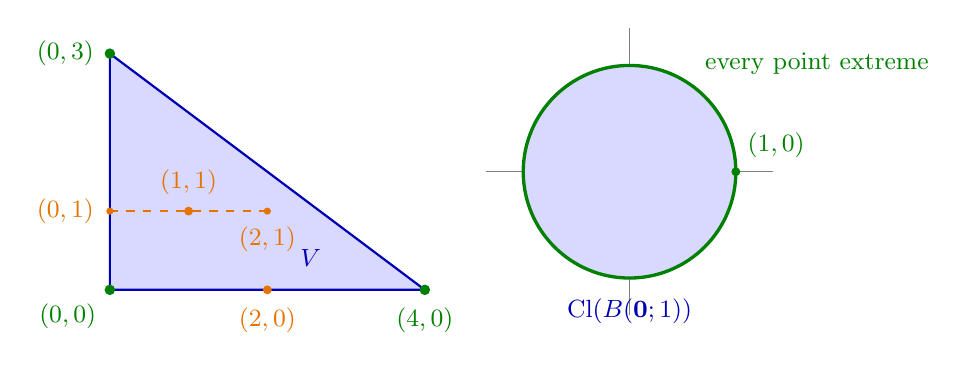
\begin{tikzpicture}[font=\small, >={Latex[length=2mm]}]
  \begin{scope}[x=1cm, y=1cm]
    \fill[blue!15] (0,0) -- (4,0) -- (0,3) -- cycle;
    \draw[blue!70!black, thick] (0,0) -- (4,0) -- (0,3) -- cycle;
    \node[blue!70!black] at (2.55,0.4) {$V$};
    \draw[orange!90!black, thick, dashed] (0,1) -- (2,1);
    \fill[orange!90!black] (0,1) circle (1.3pt) (2,1) circle (1.3pt);
    \fill[orange!90!black] (1,1) circle (1.6pt);
    \node[orange!90!black, anchor=south] at (1,1.08) {$(1,1)$};
    \node[orange!90!black, anchor=east] at (-0.08,1) {$(0,1)$};
    \node[orange!90!black, anchor=north] at (2,0.92) {$(2,1)$};
    \fill[orange!90!black] (2,0) circle (1.6pt);
    \node[orange!90!black, anchor=north] at (2,-0.1) {$(2,0)$};
    \fill[green!50!black] (0,0) circle (1.9pt) (4,0) circle (1.9pt) (0,3) circle (1.9pt);
    \node[green!50!black, anchor=north east] at (-0.05,-0.05) {$(0,0)$};
    \node[green!50!black, anchor=north] at (4,-0.1) {$(4,0)$};
    \node[green!50!black, anchor=east] at (-0.08,3) {$(0,3)$};
  \end{scope}
  \begin{scope}[xshift=6.6cm, yshift=1.5cm, x=1.35cm, y=1.35cm]
    \draw[gray, thin] (-1.35,0) -- (1.35,0);
    \draw[gray, thin] (0,-1.35) -- (0,1.35);
    \fill[blue!15] (0,0) circle (1);
    \draw[green!50!black, very thick] (0,0) circle (1);
    \fill[green!50!black] (1,0) circle (1.6pt);
    \node[green!50!black, anchor=south west] at (1.02,0.04) {$(1,0)$};
    \node[green!50!black, anchor=south west] at (0.62,0.82) {every point extreme};
    \node[blue!70!black, anchor=north] at (0,-1.1) {$\operatorname{Cl}(B(\boldsymbol{0};1))$};
  \end{scope}
\end{tikzpicture}
\end{document}
